\makeatletter
\def\input@path{{../}}
\makeatother
\documentclass[../main.tex]{subfiles}
\begin{document}
\renewcommand{\path}{3_chapter_1/}
\chapter[
CBTI
]{Alchemical Free-Energy Calculations by Multiple-replica $\lambda$-dynamics: The Conveyor Belt Thermodynamic Integration
}
\chaptermark{CBTI}
\label{ch:cbti}

\aquote{``Let us learn to dream, gentlemen, and then perhaps we
shall learn the truth.''
}
{August Kekul\'e, 1865}

\begin{abstract}
A new method is proposed to calculate alchemical free-energy differences 
based on molecular dynamics (MD) simulations, called the conveyor belt 
thermodynamic integration (CBTI) scheme.
%
As in thermodynamic integration (TI), $K$ replicas of the system are 
simulated at different values of the alchemical coupling parameter $\lambda$.
%
The number $K$ is taken to be even and the replicas are equally spaced
on a forward-turn-backward-turn path, akin to a conveyor belt (CB)
between the two physical end-states.
%
And as in $\lambda$-dynamics ($\lam$D), the $\lambda$-values associated with the 
individual systems evolve in time along the simulation.
%
However, they do so in a concerted fashion, determined by the evolution
of a single dynamical variable $\Lambda$ of period $2\pi$ controlling 
the advance of the entire CB.
%
Thus, a change of $\Lambda$ is always
associated with $K/2$ equispaced replicas moving forward and $K/2$ equispaced
replicas moving backward along $\lambda$.
%
As a result, the effective free-energy profile of the 
replica system along $\Lambda$ is periodic of period $2\pi K^{-1}$
and the magnitude of its variations decreases rapidly
upon increasing $K$, at least as $K^{-1}$ \radd{in the limit of large $K$}.
%
When \radd{a sufficient number of replicas is used}, 
these variations become small, 
which enables a complete and quasi-homogeneous coverage of the $\lambda$-range
by the replica system, without application of any biasing potential. 
If desired, a memory-based biasing potential can still be 
added to further homogenize the sampling, the preoptimization of which 
is computationally inexpensive.
%
The final free-energy profile along $\lambda$ is calculated similarly to TI,
by binning of the Hamiltonian $\lambda$-derivative as a function of $\lambda$ 
considering all replicas jointly, followed by quadrature integration. 
The associated quadrature error can be kept very low owing to 
the continuous and quasi-homogeneous $\lambda$-sampling.
%
The CBTI scheme can be viewed as a \radd{continuous/deterministic/dynamical}
%dynamical 
analog of the Hamiltonian
replica-exchange/permutation (HRE/HRP) schemes, or as a correlated 
multiple-replica analog of the \radd{$\lambda$D or} $\lambda$-local elevation umbrella 
sampling ($\lambda$-LEUS) schemes.
%
Compared to TI, it shares the advantage of the latter schemes 
in terms of enhanced orthogonal sampling, {\em i.e.} the availability of 
variable-$\lambda$ paths to circumvent conformational barriers
present at specific $\lambda$-values.
%
Compared to HRE/HRP, it permits a deterministic and continuous sampling
of the $\lambda$-range, and bypasses the need to carefully
preselect a $\lambda$-ladder \radd{and a swapping-attempt frequency}.
%
Compared to $\lambda$-LEUS, it eliminates (or drastically reduces) 
the dead time associated with the preoptimization
of a biasing potential.
%
The goal of this chapter is to provide the mathematical/physical formulation 
of the proposed CBTI scheme, along with an initial application of the method 
to the calculation of the hydration free energy of methanol.
%
\end{abstract}

\clearpage
\pagebreak

%%%%%%%%%%%%%%%%%%%%%%%%%%%%%%%%%%%%%%%%%%%%%%%%%%%%%%%%%%%%%%%%%%%%%
%% Start the main part of the manuscript here.
%%%%%%%%%%%%%%%%%%%%%%%%%%%%%%%%%%%%%%%%%%%%%%%%%%%%%%%%%%%%%%%%%%%%%
%================================================================================
\section{Introduction}
%================================================================================

%The Problem and the Solution
Newly developed advanced simulation methods are routinely tested on simple one- and two-dimensional model systems. They provide valuable insights into the theory, conceptual advantages and limitations (for examples see e.g. Refs. \cite{Huber1994, Laio2002, Christ2007, Konig2012, Koenig2020, Donnini2016, Weiss2016, Lemke2018}).
While the results of new methods are published, the implementation details may not always be available or difficult to use with different computer infrastructure.
As a result, sharing, reproducing, understanding, and comparing simulation methodologies is often cumbersome.\cite{Peng2011}
To address this issue, we have developed the Ensembler package, an easy-to-use, yet powerful platform that enables fast prototyping of new methods and comparison against existing techniques using one or two-dimensional test systems.

%Global ethical goal
Ensembler is designed following the recommendations of Stodden \textit{et al.}\cite{Stodden2016} for the enhanced reproducibility of computational methods, which includes making code publicly accessible, providing documentation, and using open licensing.\cite{Stodden2016} 
Furthermore, Ensembler uses state-of-the-art software engineering tools (i.e. git,\cite{Chacon2014} MolSSI cookie-cutter,\cite{Naden2018} and binder\cite{Binder2018}/Colab\cite{Bisong2019}) to fulfill these recommendations and enable features like continuous integration and the transparent versioning of the code. 

%-------------------------------------------------------------------------------------------------------
\subsection{Method Development}
%-------------------------------------------------------------------------------------------------------

%Why not using normal MD-Packages
The lean Python3 code\cite{Vanrossum2009} of Ensembler allows for easy prototyping of new methods and comparison against a wide range of already implemented techniques. 
In contrast, the C/C++\cite{Stroustrup1995} code of traditional high-performance molecular dynamics (MD) packages (e.g. Refs. \citenum{Berendsen1995,Lindahl2001,Vanderspoel2005,Eastman2017,Brooks2009}) is more efficient but also much more complex. 
%
%What we got
The methods currently available in Ensembler are:
\begin{itemize}
	\item \textit{Model systems}: Harmonic oscillators as well as dihedral-angle, double-well, and Lennard-Jones potential-energy functions\cite{Jones1924}
	\item \textit{Sampling algorithms}: Conjugated gradient\cite{Hestenes1952} for energy minimization, Metropolis Monte Carlo (MC),\cite{Hastings1970} leap-frog integration\cite{Vangunsteren1988} for MD, and Langevin integration\cite{Brunger1984} for stochastic dynamics (SD)
	\item \textit{Enhanced sampling techniques}: Umbrella sampling,\cite{Valleau1977} simulated tempering/temperature replica-exchange simulations,\cite{Sugita1999} local elevation/metadynamics,\cite{Huber1994, Laio2002}
	\item \textit{Free-energy methods}: Free-energy perturbation (FEP),\cite{Zwanzig1954} Bennett's acceptance ratio (BAR),\cite{Bennett1976} thermodynamic integration (TI),\cite{Kirkwood1935} enveloping distribution sampling (EDS),\cite{Christ2007, Christ2008, Christ2009} $\lambda$-EDS,\cite{Koenig2020} replica-exchange EDS (RE-EDS),\cite{Sidler2016} and conveyor-belt TI\cite{Hahn2019}
\end{itemize}

%Teaching
%-------------------------------------------------------------------------------------------------------
\subsection{Teaching}
%-------------------------------------------------------------------------------------------------------

Simple model systems can also be used for teaching MD concepts to students, as they allow to intuitively understand fundamental concepts. \cite{Pohorille2010} 
Ensembler is well suited for didactic purposes because it is not only easy to use, but supports also a range of visualizations, i.e. interactive widgets, animations, and plots, which can be embedded in Jupyter notebooks.\cite{Kluyver2016}
Example Jupyter notebooks\cite{Kluyver2016} are provided in the Ensembler GitHub repository.

%================================================================================
\section{Theory}
%================================================================================



Ensembler is implemented in Python3\cite{VanRossum2009} and available on GitHub\cite{Github2020}  (\textit{\hyperlink{https://github.com/rinikerlab/Ensembler}{rinikerlab/Ensembler}}). 
The repository is based on the template of the MolSSI cookie-cutter\cite{Naden2018} and comprises a code folder, an example folder for tutorials, example models contained in the provided Jupyter notebooks,\cite{Kluyver2016} an automatic pytest suite,\cite{Krekel2004} and the automatically generated sphinx \cite{Brandl2008} documentation. 
The code is continuously integrated via GitHub Actions,\cite{githhubAction20} providing information about code quality, test correctness, test coverage, and generation of an up-to-date documentation. 
Ensembler uses only open-source packages like the SciPy library\cite{Virtanen2020, VanDerWalt2011, Meurer2017, Mckinney2010, Hunter2007} and Jupyter notebooks.\cite{Kluyver2016} 
In the following, a user and a developer perspective are provided for the code structure. 

%-------------------------------------------------------
\subsection{User level}
%-------------------------------------------------------
 A simulation model in Ensembler consists of a potential class, a sampler class, and a system class wrapping the potential and the sampler (Figure~\ref{fig:UML-Diagramm}), and provides control over the simulation approach. 
Additionally, multiple condition classes can be added that directly influence the simulation (e.g. periodic boundary condition\cite{Cheatham1995, Leach2001} or  thermostatting\cite{Andersen1980}). 
After the construction of the system, the simulation can be started directly with the \textit{simulate} function. 
The resulting trajectory is in the form of a Pandas data frame.\cite{Mckinney2010} The trajectory is thus easily compatible with other packages like NumPy\cite{VanDerWalt2011} or scikit-learn\cite{scikit-learn} and can be stored in different formats, e.g. as .csv or .hf5 file. The system itself can be stored directly via the save function using serialization of the object with the Python package pickle.
In most cases, only a few additional lines are needed to go from simple simulation technique to more advanced one, as shown below. 

%-------------------------------------------------------
\subsection{Developer level}
%-------------------------------------------------------
The code of Ensembler is built on five interface-like base classes that allow extensive use of the inheritance concept and polymorphism \cite{Stroustrup1995} throughout the package.
These fundamental classes are \textit{potential}, \textit{sampler}, \textit{condition}, \textit{system}, and \textit{ensemble} (Figure \ref{fig:UML-Diagramm}), which can be grouped into three layers.
\textit{Potential}, \textit{sampler}, and \textit{condition classes} form the primary layer, providing different techniques to be used as components in a simulation. 
\textit{Potential classes} provide the potential-energy functions in a symbolic form using SymPy,\cite{Meurer2017} enabling automatic on-the-fly derivation and simplification of the potential-energy function. 
\textit{Sampler classes} are used to explore the potential-energy function (e.g. conjugate gradient,\cite{Hestenes1952} Metropolis MC,\cite{Hastings1970} or leap-frog\cite{VanGunsteren1988} integration). A new method can easily be implemented by inheriting from the \textit{sampler class} and overwriting a single function called \textit{step}. 
Finally, \textit{condition classes} provide additional functionalities such as thermostatting\cite{Andersen1980} and periodic boundary conditions\cite{Cheatham1995, Leach2001}). New techniques can be implemented by inheriting the base \textit{condition class} and overwriting the function \textit{apply}.
In the second layer, the first-layer components are wrapped into one \textit{system class} that executes the simulation(s) and manages the input and output. 
An optional higher-order layer is available in form of the \textit{ensemble class}, which allows the user to perform simulations with replica exchange.\cite{Sugita1999, Sugita2000, Yamauchi2017, Sidler2016a}
If additional parameters are needed in a newly designed class, the constructor of the new child class can be adapted but must call the parent constructor.


%================================================================================
\section{Computational Details}
%================================================================================

%------------------------------------------------------------
\subsection{Test System}
%------------------------------------------------------------

As an initial application of the proposed CBTI scheme, we considered here 
a relatively simple perturbation, namely the conversion of methanol
from a fully interacting molecule to a dummy skeleton (no intermolecular interactions) 
in an aqueous environment at $P=1\unit{bar}$ and $T=298.15\unit{K}$.
%
The calculations were performed using 
\radd{a modified version of the 
GROMOS11 program \cite{VA11.7,SC12.1,KU12.1} along with}
the parameters of the GROMOS-compatible 2016H66 force field\cite{HO16.1} for methanol\cite{HO11.1} (united atom, rigid bonds, flexible bond angle)
and the simple point charge (SPC) model\cite{BE81.1} for water (fully rigid).
%
Since the dummy skeleton retains the intramolecular interactions (here, only the bond angle),
the calculated free-energy change $\Delta G$ corresponds directly to minus the hydration 
free energy of methanol.


Possible issues related to the existence of a singularity\cite{SI93.1,BE94.1,ZA94.1} 
and the insufficient solute-solvent kinetic-energy exchange\cite{SH03.4,SH05.7,MO07.2,LI08.8} 
close to $\lambda=1$ were alleviated in the usual way,
by means of a soft-core scheme\cite{BE94.1} for the alchemical coupling 
and of stochastic dynamics\cite{LA08.6,VA88.1} (SD) for thermostating the solute and solvent conformational 
degrees of freedom.
%
In most CBTI simulations, the \radd{instantaneous} temperature $T_\Lambda$ of the CB advance variable
$\Lambda$ was also controlled separately by means of a 
Nos\'e-Hoover chain thermostat\cite{MA92.1} 
\radd{at 298.15 K} \revphil{(eight successive thermostat variables)},
with a coupling time $\tau_{\Lamb}$.

%------------------------------------------------------------
\subsection{Simulations Sets}
%------------------------------------------------------------

The exploration of the CBTI scheme and the comparison of its
performance with that of existing methods was carried out in five successive 
steps:
%
($1$) establishing reference TI results;
($2$) analyzing the influence of the CBTI parameters (number $K$ of replicas along with the
       mass-parameter $m_\Lambda$ and thermostat coupling time $\tau_\Lambda$ 
       of the CB advance variable);
($3$) investigating the use of a biasing potential;
($4$) examining the features of the TI-like free-energy estimator (effect of the number $J$ of integration bins and use of equations without specification of $J$);
($5$) comparing the results of CBTI with those of existing methods.


The reference TI calculations (Step 1) were performed using $K_{\mathrm{TI}}=2^n+1$ 
equidistant $\lambda$-points covering the range $[0,1]$  with $n$ = 1,2,...,7.
They involved initial configurations equilibrated for $0.2\,\mathrm{ns}$ 
starting from the equilibrated configuration at the previous $\lam$-point,
\radd{and a simulation time of $100 K_{\mathrm{TI}}^{-1}$ ns per $\lambda$-point.}
%
Each of these calculations, \radd{involving a total single-system sampling time of 100 ns},
was repeated ten times using different random initial velocities. 
%
The integration over the average Hamiltonian derivative 
was 
%then 
performed based on \refeq{ti_formula} using the Simpson quadrature rule\cite{JO10.2,BR11.5,BR11.6}.


To explore the influence of the CBTI parameters (Step 2), various 
combinations of $K$, $m_\Lambda$ and $\tau_\Lambda$ were considered in 
three series of calculations, namely:
%
($i$) the choices $m_{\Lambda}=$16,160,800,1600 or 3200$\,\mathrm{u}\,\mathrm{nm}^2$
       (where $\mathrm{u}$ stands for atomic mass unit, {\em i.e.} g mol$^{-1}$),
      along with $K=16$ replicas in the absence of thermostat coupling 
      for $\Lambda$, {\em i.e.} with $\tau_\Lambda\rightarrow\infty$;
%%      ($10\unit{ns}$ simulations of the replica system after $0.2\unit{ns}$ equilibration);
%
($ii$) the choices $\tau_\Lambda={0.05,0.1,0.5,1~\text{or}~2}\,\mathrm{ps}$
       along with $K=16$ replicas and $m_{\Lambda}=160\,\mathrm{u}\,\mathrm{nm}^2$;
%%      ($10\unit{ns}$ simulations of the replica system after $0.2\unit{ns}$ equilibration);
%
($iii$) the choices $K=8,16,32,64~\text{or}~128$
       along with 
       $m_{\Lamb}=40 K^{1/2}\,\mathrm{u}\,\mathrm{nm}^2$ 
       and $\tau_{\Lambda}=0.5\,\mathrm{ps}$;
%% ($256 K^{-1}\unit{ns}$ simulations of the replica system after $0.2\unit{ns}$ equilibration).
%
%
The parameters (and results) of these three series of simulations, including their durations $t_{\mathrm{sim}}$, are summarized  in \reftab{screen} (entries 1-15).
%
\radd{All these simulations were preceded by $0.2\unit{ns}$ equilibration}.
%
\revphil{
For the the third series (entries 11-15), $m_{\Lambda}$ was made proportional 
to $K^{1/2}$, an arbitrary parameter choice justified by arguments provided 
in \refsec{othersim}, and the five simulations relied on the 
the same total single-system sampling time of 256 ns.}
%
%
This exploration showed that the CBTI method is rather robust with respect to the choice of its parameters.
The values $K=16$, $m_\Lamb=160\,\mathrm{u}\,\mathrm{nm}^2$ and $\tau_{\Lamb}=0.5\,\mathrm{ps}$ 
were retained as 
%an optimal combination
\revphil{a good combination}
for the alchemical perturbation considered.
\radd{For comparison with the TI results of Step 1,}
ten repeats of the calculation 
involving this specific choice were performed using different random initial velocities
and 
\radd{a total single-system sampling time of 100 ns after $0.2\unit{ns}$ equilibration}.
%
%($6.25\unit{ns}$ simulations of the replica system after $0.2\unit{ns}$ equilibration, \ie{}  total $100\unit{ns}$ single-system sampling time).
%

The application of CBTI with a biasing potential (Step 3)
was investigated in the context of simulations with $K=8$ or 16, 
both with $m_{\Lamb}=40 K^{1/2}\,\mathrm{u}\,\mathrm{nm}^2$ and  $\tau_{\Lamb}=0.5\,\mathrm{ps}$.
%
For $K=8$, the biasing potential $\mathcal{B}$ (\refeq{cb_big_lam_eq_mot_bias}) was constructed 
using $N_{\mathrm{gp}}=34$ basis functions centered at equidistant grid-points \radd{$i=0,...,N_{\mathrm{gp}}-1$}
over the $\tilde{\Lamb}$-range $[0,\pi/4)$. 
%
The coefficients of the basis-functions $i$ \radd{and $N_{\mathrm{gp}}-1-i$}
\radd{with $i=0,...,N_{\mathrm{gp}}/2-1$}
were constrained to be identical, 
considering the expected even symmetry of $\tilde{P}(\tilde{\Lamb})$.
%
In terms of the CB advance variable $\Lamb$, this means that the biasing potential relied in effect on $K(N_{\mathrm{gp}}-1)=264$ local functions covering the $\Lamb$-range $[0,2\pi)$, these functions being defined by only 17 independent coefficients. 
For $K=16$, $\mathcal{B}$ 
relied on $N_{\mathrm{gp}}=18$ basis functions 
%centered 
%at equidistant grid-points 
over the $\tilde{\Lamb}$-range $[0,\pi/8)$, leading to $272$ functions over the $\Lamb$-range $[0,2\pi)$ 
%and
defined by 9 independent coefficients.
%
Second-order splines\cite{DE01.6,HA07.12} (of range $\pm 2 \delta$ with $\delta=\pi/132$ or $\pi/136$ for $K=8$ and $16$, respectively) were 
employed\cite{BI14.1} as basis functions. An initial build-up 
force constant $c_{\mathrm{LE}}=10^{-3}\,\mathrm{kJ\,mol^{-1}}$ was used, which was multiplied by a reduction factor $f_{\mathrm{red}}=0.1$ 
after each double-sweep of \radd{half} the \radd{$\tilde{\Lambda}$-range $[0,\pi K^{-1}]$.}
% 
The duration $t_{\mathrm{LE}}$ of the LE build-up phase for 
the replica system 
\radd{was $=0.15\,\mathrm{ns}$ for $K=8$ and 
$0.07\,\mathrm{ns}$ for $K=16$,
corresponding to only $1.1-1.2\,\mathrm{ns}$ 
total single-system simulation time.
%\revdavid{[DELETE:,
%which was sufficient three double-sweeps in both cases.]}
}
%
The parameters (and results) of these two simulations are summarized in \reftab{screen} (entries 16 an 17).
%
The duration $t_{\mathrm{sim}}$ of the US sampling phases for 
the replica system were $22\unit{ns}$,
corresponding to total single-system sampling 
times of $176\unit{ns}$ and $352\unit{ns}$ for $K=8$ and $16$, respectively. 
%


\begin{table}
\caption{
  \textit{Influence of the CBTI parameters in 
%\revdavid{[DELETE: unbiased]}
 simulations 
  of the aqueous methanol-to-dummy mutation at 298.15 K and 1 bar with the 
  2016H66 force field.}
%
  \revphil{This table investigates the influence of the parameters selected for the CBTI scheme
           on the temperature and dynamics of the CB advance 
           variable $\Lambda$ and on the calculated free-energy change $\Delta G$
           (for the latter, considering a constant total single-system sampling time of 100 ns).
           }
%
  \radd{For each simulation,} the successive entries are:
  the index of the simulation (sim),
  the number $K$ of replicas,
  the simulation time $t_{\mathrm{sim}}$ for the replica system,
  the mass-parameter $m_{\Lambda}$,
  the thermostat coupling time $\tau_{\Lambda}$ ($\infty$ indicates that no coupling is applied),
  the average temperature $T_\Lambda$,
  the root-mean-square fluctuation ${\sigma}_{\dot{\Lamb}}$ of $\dot{\Lambda}$,
  the autocorrelation time $\tau_{\dot{\Lamb}}$ of $\dot{\Lamb}$,
  the diffusion coefficient $D_\Lambda$ (\refeq{einstein}),
  the free-energy difference $\Delta G$ calculated using \refeq{cbti_formula} with $J=500$ (except for entry 11, $J=200$),
  the alternative free-energy difference $\Delta G_{\mathrm{alt}}$ calculated
  using \refeq{cbti_formula_app1},
  and the approximate free-energy difference $\Delta G_{\mathrm{app}}$ calculated
  using \refeq{cbti_formula_average}.
  %
  Error estimates obtained by bootstrapping \radd{(no Student $t$-factor included)} are also reported between parentheses
  for $\Delta G$, $\Delta G_{\mathrm{alt}}$
  and $\Delta G_{\mathrm{app}}$.
%
  \radd{Note that the simulations differ in terms of total single-system sampling time $Kt_{\mathrm{sim}}$.
        To enable a fair comparison, the free energy-changes and associated errors have been calculated 
        after truncating the all simulations to $100\unit{ns}$ single-system sampling time evenly distributed 
        over all replicas.}
  %
%%
%  To make the free-energy differences and associated errors comparable, the values are calculated for all simulations
%  considering only $100\unit{ns}$ single-system sampling time evenly distributed over all replicas.
%
  Associated graphs for the distributions \radd{$P(\Lambda)$ of $\Lambda$}, 
$P_{\dot{\Lambda}}$ of $\dot{\Lamb}$ and $P_{\ddot{\Lamb}}$ of $\ddot{\Lamb}$, as well as the mean-square displacements
  $d_{\Lamb}$ of $\Lamb$ and autocorrelation functions $c_{\dot{\Lamb}}$ of $\dot{\Lamb}$
  can be found in \reffigs{lam}, \reff{dynamics} \radd{and \reff{leus}, or} in Figs. \reffig{thermo:03_cvb_screen:016:1_0.01} - 
\reffig{thermo:04_cvb_thermo:128:10} \radd{and \reffig{leus:8}-\reffig{leus:16}}.
%
 Simulations $11$, $13$, $15$, \radd{$16$ and $17$} are discussed in the main text.
 The other simulations are discussed in \refsec{othersim}.
}   
\label{tab:screen}
\resizebox{\textwidth}{!}{
\begin{tabular}{*{12}{c}}
\hline
sim & $K$ & $t_{\mathrm{sim}}\,[\mathrm{ns}]$ & $m_{\Lambda} [\mathrm{u\,nm^2}]$ & $\tau_{\Lambda} [\mathrm{ps}]$ & $T_{\Lambda} [\mathrm{K}]$ & $\sigma_{\dot{\Lambda}}\,[\mathrm{ps^{-1}}]$ & $\tau_{\dot{\Lambda}}\,[\mathrm{ps}]$ & $D_{\Lambda} [\mathrm{ns^{-1}}]$ & $\Delta G\,[\mathrm{kJ\,mol^{-1}}]$ &  $\Delta G_{\mathrm{alt}}\,[\mathrm{kJ\,mol^{-1}}]$ & $\Delta G_{\mathrm{app}}\,[\mathrm{kJ\,mol^{-1}}]$ \\
%&&&&&&&&&  (\refeq{cbti_formula})  & (\refeq{cbti_formula_app1}) &  (\refeq{cbti_formula_average}) \\
\hline
    1 &    16 &    10 &    16 & $\infty$ &      308.0 &       0.40 &       0.02 &       16.7 &      21.14 (0.16) &      21.23 (0.17) &      20.21 (0.32) \\ 
    2 &    16 &    10 &   160 & $\infty$ &      297.9 &       0.12 &       0.61 &       13.2 &      21.27 (0.17) &      21.32 (0.15) &      20.29 (0.31) \\ 
    3 &    16 &    10 &   800 & $\infty$ &      296.3 &       0.05 &       1.90 &       10.2 &      21.25 (0.15) &      21.34 (0.16) &      20.27 (0.32) \\ 
    4 &    16 &    10 &  1600 & $\infty$ &      304.0 &       0.04 &       3.47 &       10.3 &      21.28 (0.15) &      21.25 (0.17) &      20.32 (0.32) \\ 
    5 &    16 &    10 &  3200 & $\infty$ &      297.7 &       0.03 &       5.63 &        7.4 &      21.23 (0.16) &      21.24 (0.18) &      20.11 (0.31) \\ 
\hline
    6 &    16 &    10 &   160 &  0.05 &      284.0 &       0.12 &       0.37 &        6.9 &      21.23 (0.16) &      21.04 (0.15) &      20.22 (0.31) \\ 
    7 &    16 &    10 &   160 &  0.10 &      291.7 &       0.12 &       0.36 &        7.4 &      21.48 (0.13) &      21.41 (0.16) &      20.47 (0.29) \\ 
    8 &    16 &    10 &   160 &  0.50 &      296.4 &       0.12 &       0.41 &        9.1 &      21.42 (0.14) &      21.48 (0.16) &      20.45 (0.30) \\ 
    9 &    16 &    10 &   160 &  1.00 &      299.4 &       0.12 &       0.49 &       12.9 &      21.57 (0.16) &      21.48 (0.17) &      20.59 (0.30) \\ 
   10 &    16 &    10 &   160 &  2.00 &      296.8 &       0.12 &       0.56 &       13.1 &      21.48 (0.13) &      21.73 (0.15) &      20.45 (0.29) \\ 
\hline
   11 &     8 &    32 &   113 &  0.50 &      298.4 &       0.15 &       0.23 &        4.4 &      21.69 (0.40) &      21.69 (0.44) &      15.65 (0.31) \\ 
   12 &    16 &    16 &   160 &  0.50 &      298.3 &       0.12 &       0.41 &       10.2 &      21.42 (0.16) &      21.48 (0.17) &      20.45 (0.33) \\ 
   13 &    32 &     8 &   226 &  0.50 &      300.6 &       0.10 &       0.38 &        6.2 &      21.44 (0.14) &      21.33 (0.15) &      21.34 (0.32) \\ 
   14 &    64 &     3 &   320 &  0.50 &      297.2 &       0.09 &       0.31 &        2.5 &      21.32 (0.14) &      21.27 (0.14) &      21.29 (0.30) \\ 
   15 &   128 &     2 &   452 &  0.50 &      304.1 &       0.08 &       0.24 &        2.3 &      21.43 (0.12) &      21.61 (0.14) &      21.41 (0.32) \\ 
\hline
   16 &     8 &    22 &   113 &  0.50 &      296.4 &       0.15 &       0.43 &       15.3 &      21.48 (0.16) &      21.61 (0.17) &      19.65 (0.34) \\ 
   17 &    16 &    22 &   160 &  0.50 &      299.3 &       0.12 &       0.43 &        9.4 &      21.30 (0.13) &      21.43 (0.16) &      20.61 (0.34) \\ 
\end{tabular}
}
\end{table}



%
To examine the features of the TI-like free-energy estimator (Step 4),
the number $J$ of integration bins
used in the rectangular quadrature to calculate $\Delta G$ (\refeq{cbti_formula}) was varied  considering the simulations of Steps 2 and 3 above (17 simulations of \reftab{screen}). 
%
%
%
The resulting $\Delta G$ values were also compared to those 
of the variants $\Delta G_{\mathrm{alt}}$ (\refeq{cbti_formula_app1}) 
and $\Delta G_{\mathrm{app}}$ (\refeq{cbti_formula_average}) \revphil{proposed in \refsec{CH2C}}.



Finally, the results of the CBTI simulations were compared to 
those of other methods (Step 5), namely TI or HRE using Simpson quadrature
as estimator as well as TI using EXTI and MBAR as estimator.
%
%
%XXX MOVED FROM BELOW
%Finally, the results of CBTI were compared to those of existing methods,
%namely TI and HRE using Simpson quadrature as free-energy estimator or TI
%using EXTI and MBAR.
%
\radd{For Simpson quadrature,} the TI simulations relied on $K_{\mathrm{TI}}=3,5,9,17,65$ or 129 equispaced $\lam$-points,
and the HRE simulations relied on $K_{\mathrm{HRE}}=17,33~\text{or}~65$ equispaced replicas 
with exchange attempts every $\tau_{\mathrm{HRE}}=0.2\,\mathrm{ps}$.
%
\radd{The use of EXTI and MBAR was explored based on TI-like
simulations relying on $K_{\mathrm{TI}}=9$ and $17$ equispaced $\lam$-points.
%
For EXTI, the \radd{average} Hamiltonian derivative was extrapolated 
%\revdavid{[DELETE: using OSP ]
}
during the $K_{\mathrm{TI}}$ simulations to 129 equispaced virtual $\lam$-points,
and the latter 129 values used in the Simpson quadrature.
%
For MBAR, the Hamiltonian was calculated at 129 equispaced virtual
$\lam$-points considering all the configurations sampled in the $K_{\mathrm{TI}}$, 
and the data combined using the MBAR equation\cite{SH08.7} as implemented in pymbar\cite{CH17.16}.
%
All the above comparisons were performed at a total single-system 
sampling time of $100\unit{ns}$ distributed evenly over all replicas.



\radd{Error bars on the calculated $\Delta G$ values
were estimated in two different ways.}
%
For the \radd{calculations involving ten repeats (all TI calculations plus one CBTI simulation),
%
the standard deviation $\sigma$ of the mean was calculated 
by scaling that of the ten estimates by the square-root of nine,
and the error $\epsilon$ on the mean was calculated 
as $\epsilon=2.262 \sigma$, where $2.262$
is the Student $t$-factor\cite{ST08.9} for nine degrees of freedom 
and a two-sigma confidence interval of $95\%$.
}
%
For the \radd{individual calculations that were not repeated},
the statistical error was estimated
by bootstrapping\cite{EF79.1,EF98.1} \radd{(no Student $t$-factor included)} 
\radd{using 100 bootstrap samples.
%
If $K$ replicas (CBTI) or $\lambda$-points (all other methods) 
have generated as many sets of $L$ data points, a sample consists 
here of $K$ sets of  $L$ data points selected randomly 
(possibly multiple times) from the $K$ original data sets.
}
%
\revphil{Note that for TI/EXTI and TI/MBAR, it is essential to perform 
the bootstrapping based on the data from the $K_{\mathrm{TI}}$ real 
$\lambda$-points, and not from the $129 K_{\mathrm{TI}}$ predicted values
(the latter procedure would result in underestimated errors 
due to correlation in the derived data).}
%
\radd{The bootstrapping error will only be accurate 
provided that the data from the simulations, written to file every $2\unit{ps}$, 
is uncorrelated in time.}
%
\radd{Normalized autocorrelation} functions and characteristic times for the \radd{average} Hamiltonian derivative
in the different TI-simulations are provided in
%
\reffig{ti:tcf} and \reftab{tcf} to support this assumption. 



%
%> The result of EXTI is now 21.12 (0.14) kJ mol^-1, which is in about the same
%> order of magnitude as all other methods.
%>
%> There is still a little issue:
%> I used 100 bootstrap samples of the simulated points and predicted the
%> non-simulated points from the same bootstrap sample (as discussed last
%> Thursday). Now, I calculated the error in two different ways:
%> - I took the 100 bootstrap samples per simulated point and calculated the
%> error on the dH/dl on all 129 (predicted) lam-points. Then I calculated the
%> error on the final Delta G by error propagation. *This still leads to an
%> error which is much smaller (0.03kJ mol^-1)* I assume, that the error
%> propagation is not correct because it neglects the cross-correlation between
%> the lambda-points which is definitely there because of the prediction.
%> - For each bootstrap sample of all simulated lam-points, I calculated a dHdl
%> curve and a Delta G. Then the bootstrap error is the standard deviation  of
%> the 100 Delta G values. This yields to the 0.14 kJ mol^-1. This is cleaner,
%> you don't have to do error propagation and it is the same way as I calculated
%> the error for the other methods.
%>
%> In the plots and tables I used error #2, which is more trustworthy in my
%> opinion. I will have a look whether I can improve the error propagation that
%> error #1 is also in the same range.
%>
%>
%






%------------------------------------------------------------
\subsection{Simulation Parameters}
%------------------------------------------------------------


The simulations involved a cubic computational box containing one methanol
and 1000 water molecules under periodic boundary conditions
in the isothermal-isobaric ensemble at 
$P=1\unit{bar}$ and $T=298.15\unit{K}$.
%
They were performed using SD 
by integrating the Langevin equation of motion\cite{LA08.6}
using the leap-frog scheme\cite{HO70.1} (SD variant\cite{VA88.1}) with a timestep $\Delta t=2\,\mathrm{fs}$
and a friction coefficient $\gamma=10\,\mathrm{ps^{-1}}$.
%
Since the kinetics of the system is irrelevant in this work, SD instead of thermostated MD was used to 
avoid problems related to insufficient solute-solvent kinetic-energy exchange\cite{SH03.4,SH05.7,MO07.2,LI08.8}
close to $\lambda=1$ (dummy-skeleton state).
The value of $\gamma$ corresponds 
%effectively 
to the  coupling time of $0.1\unit{ps}$
commonly employed in GROMOS simulations\cite{VA96.1,VA11.7} relying on a weak-coupling\cite{BE84.1} thermostat.
%
The average pressure was maintained close to its reference value
by isotropic weak coupling\cite{BE84.1} using a molecular virial, 
a coupling time $\tau_{P}=0.5\,\textrm{ps}$
and a compressibility $\kappa=4.575\cdot10^4\,\mathrm{kJ}\,\mathrm{mol}^{-1}\,\mathrm{nm}^{-3}$
as commonly used in GROMOS for aqueous biomolecular systems\cite{VA96.1,VA11.7}.
%
The bond rigidity  of methanol and the full rigidity of water were enforced by
application of the SHAKE algorithm\cite{RY77.1} with a relative 
geometric tolerance of $10^{-4}$. 
%
The energies and 
%\radd{average} 
Hamiltonian derivatives
were written to file every $2\unit{ps}$ for analysis.
%


The non-bonded interactions were handled by means of a molecule-based
twin-range cutoff scheme\cite{BE86.3}
with short- and long-range cutoff distances set
to $0.8$ and $1.4\unit{nm}$, respectively, and an update frequency of
5 timesteps for the short-range pairlist and intermediate-range
interactions. The molecule center was the center of geometry for methanol and the oxygen atom for water.
A reaction-field correction\cite{BA73.1,TI95.1} was applied to account for the mean effect of the electrostatic interactions beyond the long-range cutoff distance, using a relative
dielectric permittivity of $61$ as appropriate for the SPC model~\cite{HE01.1}.
%
To alleviate issues related to the existence of a singularity\cite{SI93.1,BE94.1,ZA94.1} 
close to $\lambda=1$ (dummy-skeleton state), the alchemical transformation
relied on a soft-core scheme\cite{BE94.1},
applied with the parameters $\alpha_{\mathrm{LJ}}=0.5$ and $\alpha_{\mathrm{CRF}}=0.5\,\mathrm{nm}^2$.
%

For the CBTI calculations, the propagation of the $\Lamb$ variable
(\refeq{cb_big_lam_eq_mot}) preceded that 
of the conformational degrees of freedom, and was performed with the same 
timestep $\Delta t$.
%
More precisely, the following 
leap-frog steps were carried out in sequence:
$\dot{\Lamb}(t-\Delta t/2) \rightarrow \dot{\Lamb}(t+\Delta t/2)$,
$\Lamb(t) \rightarrow \Lamb(t+\Delta t)$,
calculate $\lamv$ from $\Lambda$ using \refeq{cb_lam_of_big_lam},
$\dot{\rv}(t-\Delta t/2) \rightarrow \dot{\rv}(t+\Delta t/2)$
and
$\rv(t) \rightarrow \rv(t+\Delta t)$.
%
Unless otherwise specified (explorative simulations), 
\radd{the CBTI simulations 
relied on a
mass-parameter $m_\Lambda$
set to $m_{\Lamb}=40 K^{1/2}\,\mathrm{u}\,\mathrm{nm}^2$,
%where $K$ is the number of replicas, and
%the temperature of the $\Lambda$-variable was controlled separately
%by means of a Nos\'e-Hoover chain thermostat\cite{MA92.1}
%involving eight successive thermostat variables at a reference temperature of $298.15\unit{K}$
%and with a 
on a coupling time $\tau_{\Lambda}$ set to $0.5\unit{ps}$,
and 
%
%And unless otherwise specified 
%(investigation of the effect of $J$ and unbiased CBTI simulation with $K=8$), 
on the use of $J=500$ bins 
for evaluating
$\Delta G$ based on \refeq{cbti_formula}
($J=200$ for the unbiased simulation with $K=8$).
}


%------------------------------------------------------------
\subsection{Trajectory Analysis}
%------------------------------------------------------------

The dynamics of the replica system in the CBTI simulations was characterized by monitoring
the distribution $P$ of the $\Lambda$ variable,
the average temperature $T_{\Lamb}$, 
the distribution $P_{\dot{\Lamb}}$ of $\dot{\Lamb}$, 
the associated root-mean-square fluctuation $\sigma_{\dot{\Lamb}}$, 
the \radd{normalized} autocorrelation function $c_{\dot{\Lambda}}$ of $\dot{\Lamb}$, 
the associated autocorrelation time $\tau_{\dot{\Lambda}}$, 
\radd{the mean-square displacement $d_{\Lamb}$ of $\Lamb$ as a function of time},
the associated diffusion coefficient $D_{\Lambda}$, 
and 
the distribution $P_{\ddot{\Lambda}}$ of $\ddot{\Lambda}$.
%
%
%


The distribution $P_{\dot{\Lamb}}$ of $\dot{\Lamb}$ can be compared to the analytical one-dimensional Maxwell-Boltzmann velocity distribution\cite{MA60.1}
%
\beq{ana_vel}
P^{\mathrm{MB}}_{\dot{\Lamb}}(\dot{\Lamb})=\left ( \frac{\beta m_{\Lamb}}{2\pi} \right )^{\frac{1}{2}} \mathrm{e}^{-\frac{\beta m_{\Lamb}}{2} \dot{\Lamb}^2}.
\eeq
%


The diffusion coefficient $D_{\Lamb}$ was calculated from the mean-square displacement $d_{\Lamb}$ of $\Lamb$ as a function of time $t$ according to the one-dimensional Einstein equation\cite{EI05.1}
%
\begin{multline}
  \label{eq:einstein}
  D_{\Lamb}=\lim\limits_{t\rightarrow \infty} \frac{d_{\Lamb}(t)}{2t} \\
  \text{with} \qquad d_{\Lamb}(t)=\left \langle \left[\Lamb(\tau + t) -\Lamb (\tau)\right ]^2 \right \rangle_{t},
\end{multline}
%
where $\langle \cdot\cdot\cdot \rangle_{t}$ denotes averaging over $\tau$ (all possible time origins) at constant $t$. Note that this equation must be applied to the unbounded variable $\Lamb$, \ie{}  without refolding to the reference interval $[0,2\pi)$.
The infinite-time limit was replaced in practice by a linear least-squares fit over the time range 0 to $0.15\unit{ns}$.
%
\revphildel{[-- Redundant paragraph removed --]}


%To investigate the influence of the number $J$ of bins used 
%to calculate the free-energy differences $\Delta G$ in CBTI according to \refeq{cbti_formula},
%this number was systematically increased from 1 to $J_{\mathrm{max}}$ in increments ranging 
%from 10 to 1000, where $J_{\mathrm{max}}$ is the highest value of $J$ for which empty bins never occur.
%%
%%
%\revphil{The estimates} $\Delta G_{\mathrm{alt}}$ and $\Delta G_{\mathrm{app}}$ were also calculated \revphil{for comparison},
%using \refeqs{cbti_formula_app1} and \refeqn{cbti_formula_average} \revphil{of Appendix C}.
%%The latter one is only expected to be accurate for quasi-homogeneous sampling of the $\lam$-range. 
%%
%


All the graphs presented in this chapter were generated with Python (www.python.org) and the Matplotlib library.\cite{HU07.7}



%================================================================================
\section{Results and Discussion}
%================================================================================

%-------------------------------------------------------------------------------------------------------------------------
\subsection{Simple Simulations}
%-------------------------------------------------------------------------------------------------------------------------
In the following, simple code examples are shown to introduce the usage of Ensembler. In addition, an application example is provided to illustrate the use of Ensembler for teaching about free-energy methods. 
The code for these examples can be found in the GitHub repository \textit{\hyperlink{https://github.com/rinikerlab/Ensembler}{https://github.com/rinikerlab/Ensembler/examples}}.
\begin{figure}[h!]
	\centering
	\begin{subfigure}{0.85\textwidth}
		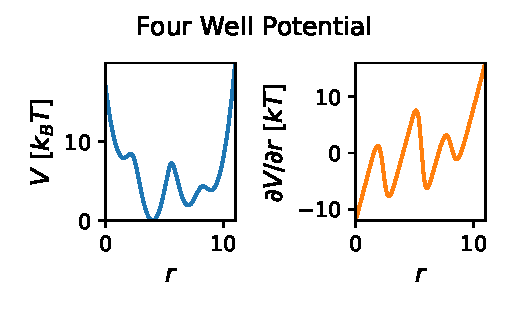
\includegraphics[width=\linewidth, height=1.75in]{fig/codeExamples/four_well.pdf} 
		\caption{}
	\end{subfigure}\\
	\begin{subfigure}{0.85\textwidth}
		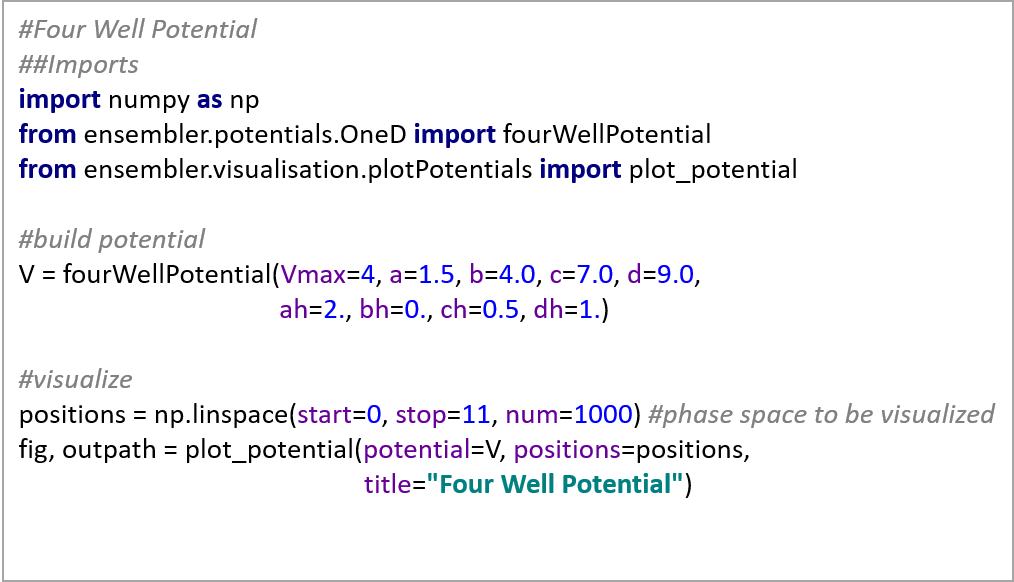
\includegraphics[width=\linewidth, height=1.75in]{fig/codeExamples/Potential_code.png}
		\caption{}
	\end{subfigure}
	\caption{A four-well potential-energy surface visualized by the standard visualization function of Ensembler. (a) Potential-energy function (blue) and the automatically generated spatial gradient (orange) over a given coordinate range. (b) Source code to define the potential-energy function and the coordinate range to be visualized. These parameters are passed to the built-in plotting function in the \textit{potential classes} of Ensembler.}
	\label{fig:code_example_potential}
\end{figure}

In typical applications of Ensembler, the user selects a potential-energy function from the available ones. In the following example, a potential-energy function with four wells is selected and initialized with chosen parameters. 
To sample this four-well potential-energy function with stochastic dynamics (SD),\cite{Brunger1984} the sampling method is instantiated and passed to the \textit{system class}, which controls the execution of the simulation. 
The simulation is performed by calling the function \textit{simulate} with the desired number of simulation steps passed as parameter. 
Subsequently, the results can be visualized using the built-in visualization functions that are compatible with the \textit{simulation class} of Ensembler.  
As can be seen in Figure \ref{fig:code_example_simulations}a, the energy barriers between the different minima were not crossed during the chosen simulation length. 
To overcome the sampling issue, enhanced sampling techniques can be employed.\cite{Pohorille2010} 
In this example, local elevation\cite{Huber1994}/metadynamics\cite{Laio2002} is used to overcome the energy barriers (Figure \ref{fig:code_example_simulations}b).
The method adds a time-dependent biasing potential to the system, i.e. it adds a Gaussian biasing potential to positions that were already visited such that they become energetically less favorable. This decreases the likelihood of visiting known positions again. 
The enhanced sampling technique can be applied by adding a single line of code compared to the previous simulation (Figure \ref{fig:code_example_simulations}c).

\begin{figure}[h]
	\centering
	\begin{subfigure}{\textwidth}
		\caption{Standard Langevin Simulation}
		\centering
		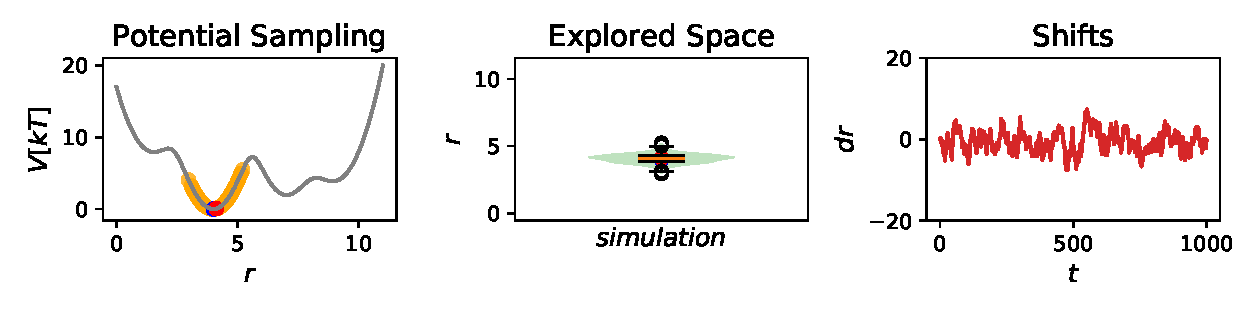
\includegraphics[width=0.85\linewidth]{fig/codeExamples/langevin_simulation.pdf} 
	\end{subfigure}
	\vspace{2.5mm}
	\begin{subfigure}{\textwidth}
		\caption{Langevin Simulation with Local Elevation/Metadynamics}
		\centering
		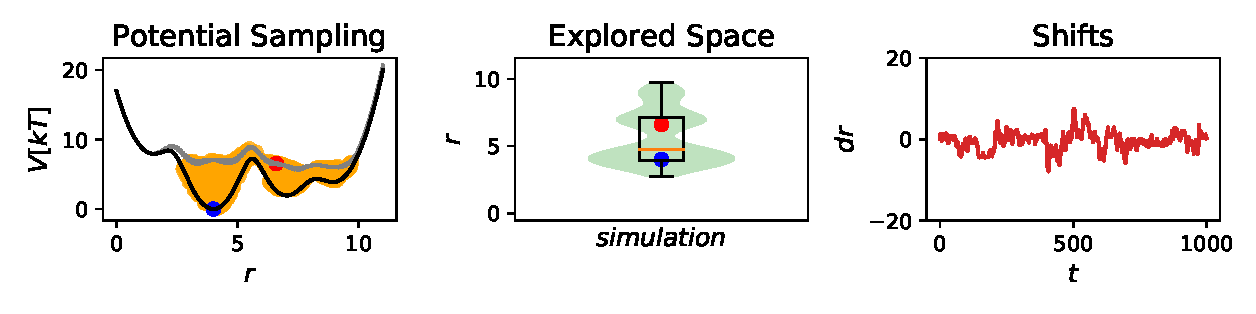
\includegraphics[width=0.85\linewidth]{fig/codeExamples/metaDynamics_simulation.pdf}
	\end{subfigure}
	\vspace{2.5mm}
	\begin{subfigure}{\textwidth}
		\caption{Example Source Code}
		\centering
		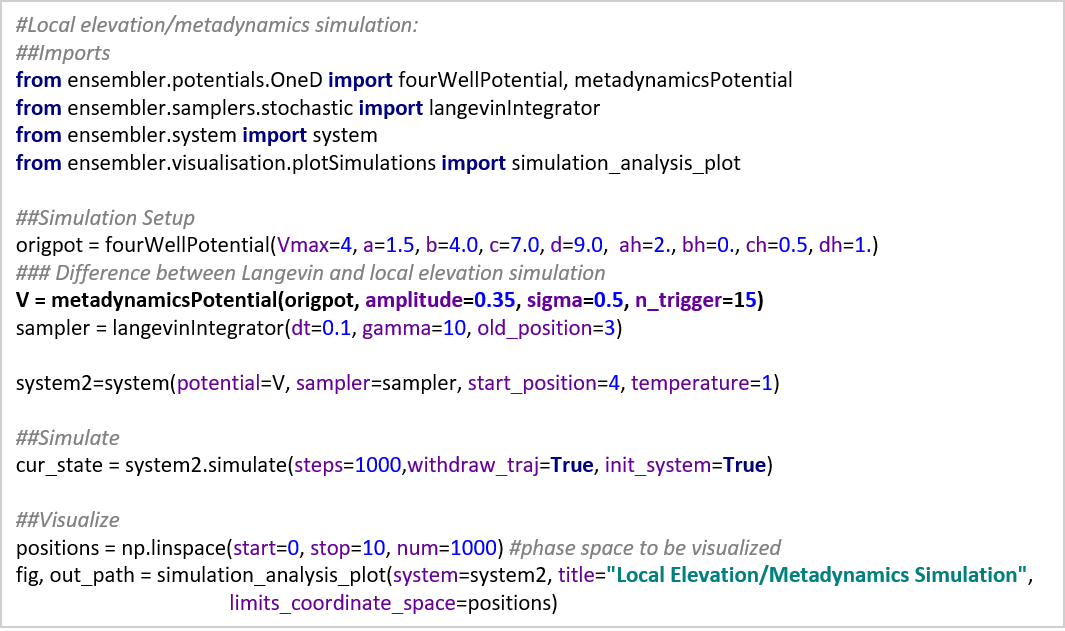
\includegraphics[width=0.85\linewidth]{fig/codeExamples/Simulation_code.png}
	\end{subfigure}
\caption{Langevin simulation of a four-well potential energy-function. Results when sampling (1000 steps) with the standard SD integrator (a) or with local elevation\cite{Huber1994}/metadynamics\cite{Laio2002} (b). The left panel shows the potential-energy surface (black), the sampled range (orange), as well as the start point (blue) and end point (red). The middle panel shows the sampled space as a violin/box plot with the start point (blue) and end point (red). The right panel shows the shift $\Delta r_t$ = $r_{t+1}$ - $r_t$ as a function of simulation time $t$.
	(c) Source code to perform the simulations. First, the four-well \textit{potential class} and the Langevin \textit{sampler class} are initiated. Next, they are wrapped by a \textit{system class}, which executes the simulation. Visualizations are generated with a built-in functions. Note that only one line has to be added to use the enhanced sampling technique (marked in bold).}
\label{fig:code_example_simulations}
\end{figure}

\FloatBarrier
\clearpage

%-------------------------------------------------------------------------------------------------------------------------
\subsection{Free-Energy Calculation}
%-------------------------------------------------------------------------------------------------------------------------

Free-energy calculation is an important field in computational chemistry because free-energy differences govern the outcome of processes in nature, e.g. protein-ligand binding or polymer formation.\cite{Christ2009, Hansen2014, Cournia2020, Armacost2020} 
%
The calculation of alchemical free-energy differences with Ensembler is exemplified with a mutation of the equilibrium position of a one-dimensional harmonic oscillator (Figure \ref{fig:FE_sampling}a).
This mutation corresponds to a change of a covalent bond type at the terminus of a linear molecule and can be calculated analytically (Table \ref{tab:FE_results}).
In practical applications, however, it is usually not possible to calculate the free-energy difference analytically. In these cases, MD-based simulation techniques can be employed.
In the following, the sampling of the two end states of the model system and the results of the free-energy calculation with different methods are discussed. For more details, we refer to the Jupyter notebook in the Ensembler GitHub repository.

A simple free-energy method is to simulate one end state and estimate the free-energy difference with the Zwanzig equation.\cite{Zwanzig1954} The quality of the result depends on a sufficient phase-space overlap between the two end states.\cite{Konig2018}
Alternatively, one can simulate both end states separately and use BAR\cite{Bennett1976} (Figure \ref{fig:FE_sampling}a), yielding more converged results.\cite{Konig2018}
If the phase-space overlap between the two end states is not sufficient, more advanced sampling methods are necessary to obtain converged free-energy differences.
%
\begin{figure}[h]
	\centering
	\begin{subfigure}{.85\textwidth}
		\caption{}
		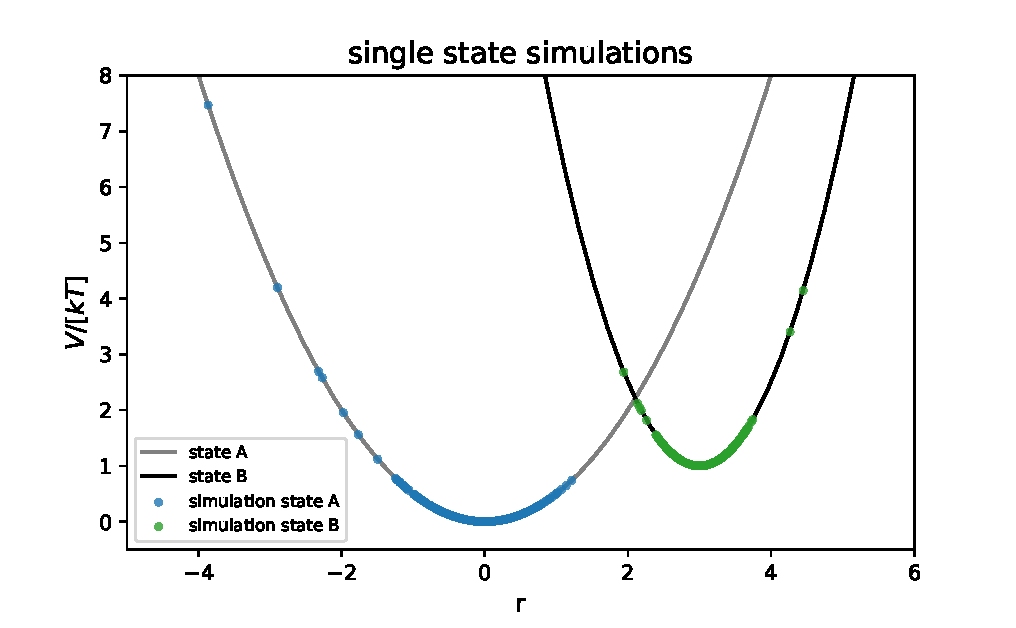
\includegraphics[width=\linewidth]{fig/FE_example/freeEnergyPertubation.pdf} 
	\end{subfigure}\\
	\begin{subfigure}{.85\textwidth}
		\caption{}
		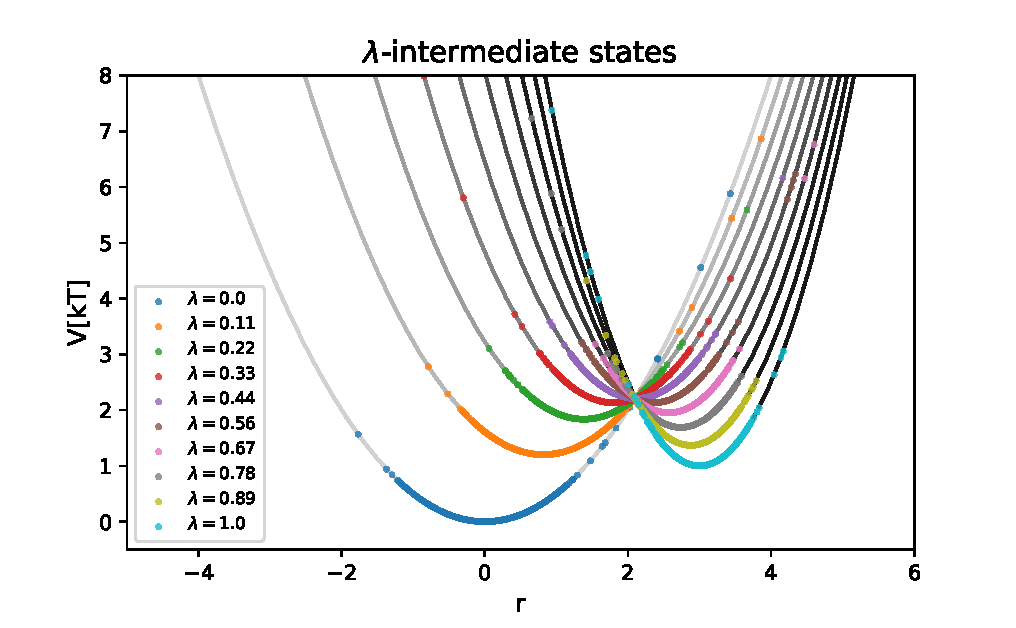
\includegraphics[width=\linewidth]{fig/FE_example/linear_coupled.pdf} 
	\end{subfigure}
	\caption{Illustration of different free-energy methods implemented in Ensembler (part I). (a) For FEP\cite{Zwanzig1954} and BAR\cite{Bennett1976}, the two end states (grey and black) are sampled separately (green and blue). (b) To increase the phase-space overlap, the two end states can be coupled as a linear combination of their Hamiltonians using a coupling parameter $\lambda$. This allows the generation of intermediate states (grey to black) and sampling of those (colored points).}
	\label{fig:FE_sampling}
\end{figure}
%
\begin{figure}[h]
	\centering
	\begin{subfigure}{.85\textwidth}
		\caption{}
		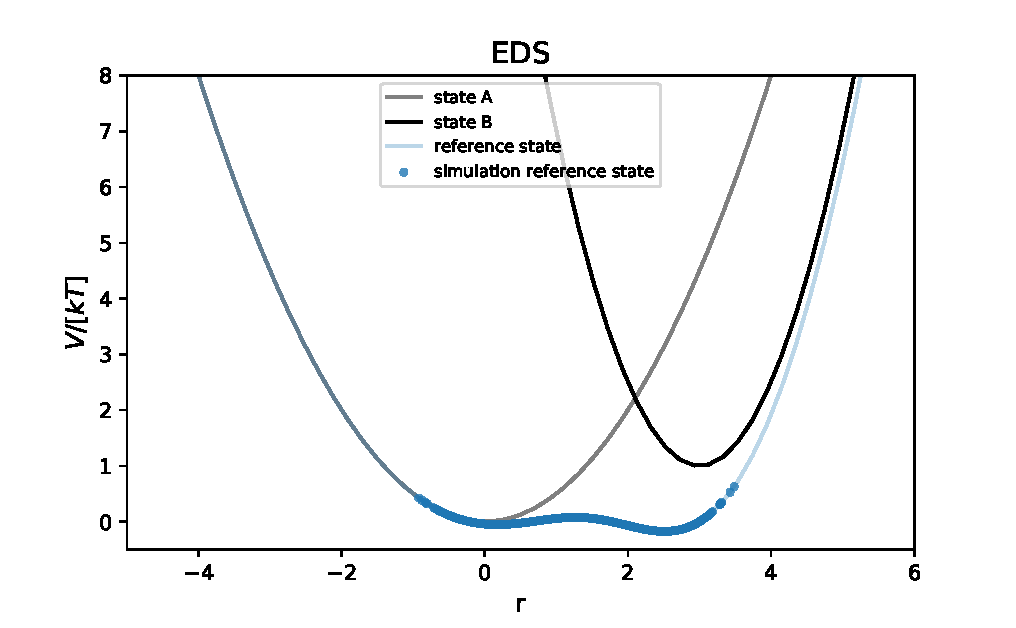
\includegraphics[width=\linewidth]{fig/FE_example/EDS_sampling.pdf} 
	\end{subfigure}\\
	\begin{subfigure}{.85\textwidth}
		\caption{}
		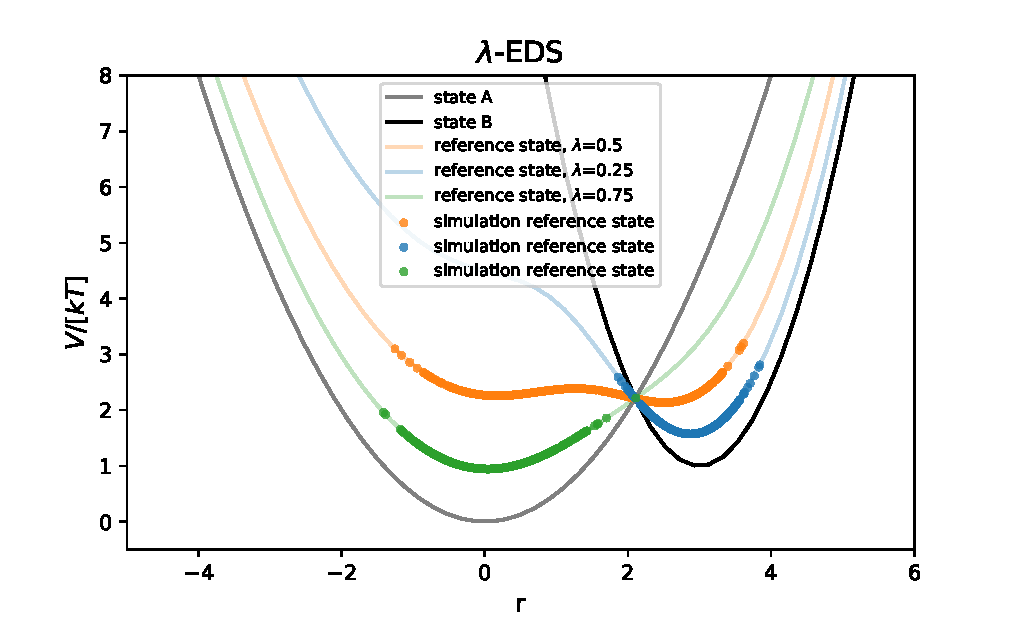
\includegraphics[width=\linewidth]{fig/FE_example/hlEDS_sampling.pdf} 
	\end{subfigure}
	\caption{Illustration of different free-energy methods implemented in Ensembler (part II). (a) An alternative method is EDS,\cite{Christ2007, Christ2008, Christ2009} where a reference-state Hamiltonian (blue line) is sampled (blue points), which envelopes the end states. By setting the reference-state parameters to $s$~=~0.3 and energy offsets~=~[0,0], all relevant phase-space regions can be sampled. (b) A recently developed approach called $\lambda$-EDS\cite{Koenig2020} introduces a $\lambda$-dependence in the EDS method (blue, orange and green line). Colored points indicate sampling. The reference-state parameters were set to $s$~=~0.3 and energy offsets~=~[0,0], and three different lambda values 0.25,0.5, 0.75 were chosen.}
	\label{fig:FE_samplingb}
\end{figure}
%%linear coupling
One possibility to increase the phase-space overlap is to generate intermediate states as a linear combination of the two end states $A$ and $B$ with the coupling parameter $\lambda$, i.e. $H(\lambda) = (1-\lambda) H_A + \lambda H_B$, such that $H(\lambda=0) = H_A$ and $H(\lambda=1) = H_B$.
The intermediate states are positioned at discrete $\lambda$-points between 0 and 1 (Figure \ref{fig:FE_sampling}b).\cite{Valleau1972, Straatsma1991} 
The free-energy difference can be estimated using FEP\cite{Zwanzig1954} or BAR\cite{Bennett1976} as the path over all intermediates, or with TI\cite{Kirkwood1935} as the integral along $\lambda$. 

%% EDS
Another elegant free-energy method is EDS,\cite{Christ2007, Christ2008} where a reference-state Hamiltonian $H_r$ is sampled. $H_r$ is constructed as a log-sum of the Hamiltonians of the two (or more) end states, guaranteeing the phase-space overlap of the reference state with all end states,
\begin{equation}
H_R = - \frac{1}{\beta s} \ln( e^{(- \beta s (H_A - E^R_A)}) +e^{(- \beta s (H_B - E^R_B)}),
\end{equation}
where $1/\beta=k_{B}T$, $k_B$ being the Boltzmann constant and $T$ the absolute temperature.
$H_R$ can be optimized for sampling using two kinds of parameters: The smoothing parameter $s$ lowers the energy barriers between the end states, whereas the energy offsets $E^R$ ensure equal weighting of all end states. In our example, both end states are sampled sufficiently during the EDS simulation with $s=0.3$ and the energy offsets $E^R=[0,0]$ (Figure \ref{fig:FE_sampling}c). Subsequently, the Zwanzig equation\cite{Zwanzig1954} is used to obtain the free-energy difference between the end states.\cite{Christ2007, Christ2008}
%hybrid coupling l-EDS
Recently, a hybrid form of EDS and $\lambda$-coupling was introduced, termed $\lambda$-EDS.\cite{Koenig2020} At $\lambda=0$ or $1$, the $H_R$ is equal to the Hamiltonians of the respective end states, while conventional EDS is recovered with $\lambda$=0.5 (except for an offset).\cite{Koenig2020}
$\lambda$-EDS allows for a $\lambda$-weighting of the exponential terms in the EDS equation. In the example in Figure \ref{fig:FE_sampling}d, the same reference-state parameters were used as before.

%final comparison
All free-energy calculations discussed above were performed with Ensembler for a total of 10'000 Monte Carlo (MC)\cite{Hastings1970} steps, and each simulation was repeated five times.
The simulation results listed in Table \ref{tab:FE_results} show that larger errors are obtained without intermediate states due to insufficient phase-space overlap.
Using ten $\lambda$–intermediate states together with TI gave the best result, however, this approach is also the computationally most expensive one (i.e. ten separate simulations). s
EDS and $\lambda$-EDS, on the other hand, yielded also good results, while requiring only one simulation (given a set of suitable reference-state parameters). 
We refer to the Jupyter notebook in the Ensembler GitHub repository for the source code, more detailed information on these methods as well as additional methods like conveyor-belt TI\cite{Hahn2019} and RE-EDS,\cite{Sidler2016, Sidler2017} which combine enhanced sampling and free-energy methods.
\begin{table}[ht]
	\centering
	\caption{Estimated free-energy difference for the model system shown in Figure \ref{fig:FE_sampling}. Sampling was performed with Monte Carlo method (MC)\cite{Hastings1970} for 10'000 steps in each simulation. Each calculation was replicated five times and the averaged result is shown together with the standard deviation.
		The duration of the computations (without visualizations) was estimated directly in the Jupyter notebook and is given relative to the FEP simulation (absolute duration = 2.0 seconds). The performance was tested on a Lenovo Thinkpad T420s with an Intel i5-2520 ($2.5~\text{GHz}$) CPU and $8~\text{GB}$ RAM. The RAM usage for the full Jupyter notebook execution was in total $578~\text{MB}$.}
	\label{tab:FE_results}
	\resizebox{\columnwidth}{!}{%
		\begin{tabular}{l|r | c| r r}
			Method & Average $\Delta$F & Deviation from & \multicolumn{2}{c}{Speed (rel. to FEP)}\\
			&      [$k_B T$]  & analytical result [$k_B T$] & Simulation & Analysis \\
			\hline
			\textit{analytical} & 1.275 & - & - & -  \\
			FEP\cite{Zwanzig1954} & $6.579 \pm  1.009$ & 5.305 & 1.0 & 0.1  \\
			BAR\cite{Bennett1976} & $2.437 \pm  0.500$ & 2.437 & 3.0 & 2.1 \\
			FEP 10-$\lambda$-points &  $1.406 \pm 0.431$ & 0.131 & 14.0 & 0.7 \\
			TI\cite{Kirkwood1935} 10-$\lambda$-points& $1.242 \pm 0.015$ & 0.033 & 14.0 & 0.04\\
			EDS\cite{Christ2007, Christ2008, Christ2009} &  $0.958 \pm 0.110$ & 0.317 & 2.4 &  0.2 \\
			$\lambda$-EDS\cite{Koenig2020} $\lambda=0.5$ & $ 0.987 \pm  0.111$ & 0.287 & 3.1 & 0.2\\
		\end{tabular}
	}
\end{table}


\clearpage
\newpage

%================================================================================
\section{Conclusion}
%================================================================================

In the present chapter, we proposed a new method called 
conveyor belt thermodynamic integration (CBTI)
to calculate alchemical free-energy differences based on 
MD simulations.
%
This approach borrows and combines ideas from
thermodynamic integration\cite{KI33.1,KI34.2,KI35.1} (TI),
\radd{replica exchange\cite{SU99.1,FU02.2,ZH16.2} (HRE) or permutation\cite{IT13.1,IT13.2,YA17.2} (HRP),}
and $\lambda$-dynamics\cite{KO96.1,DA01.7,GU03.1,KN09.1,KN11.2,DO11.2,AR15.2,HA17.1} ($\lambda$D),
along with the real-life working principle
of the funicular.
%

%
In CBTI, one simulates in parallel a set of $K$ 
\radd{equally spaced} replicas
(with $K$ even) on a forward-turn-backward-turn 
path along the alchemical coupling variable $\lambda$, 
akin to a conveyor belt (CB) between the two physical end 
states.
%
Because the $\lambda$-forces (Hamiltonian $\lambda$-derivative)
exerted by the individual replicas on the CB largely 
compensate each other, the overall $\Lambda$-force on 
the CB advance variable $\Lambda$ becomes increasingly 
small when $K$ is made increasingly large (residual free-energy
barriers decreasing at least as $K^{-1}$ \radd{in the limit of large $K$}, as shown in \refsec{quad}).
%
As a result, \radd{for a sufficient number $K$}, quasi-homogeneous
sampling of the $\lambda$-range can be achieved
without application of any biasing potential.
%
If a \radd{smaller $K$} is employed, a memory-based biasing potential 
can still be added to further homogenize the sampling,
the preoptimization of which is computationally inexpensive.
%
The results of a CBTI simulation (whether biased or not) can be analyzed similarly to TI,
by binning of the \radd{average} Hamiltonian $\lambda$-derivative as a function 
of $\lambda$ considering all replicas jointly, followed 
by quadrature integration. 
%
In this case, the continuous and quasi-homogeneous sampling of the $\lam$-range permits to use a large number of bins,
thereby essentially eliminating quadrature errors.

As a first application, 
the CBTI scheme was employed here to calculate the 
hydration free energy of methanol.
%
It was shown that the method is rather robust with respect 
to the choice of its parameters ($K$ as well as the mass-parameter $m_{\Lamb}$ and thermostat coupling time $\tau_\Lamb$ of the CB), the 
most important sensitivity being relative to $K$.
%
Upon increasing $K$, the distribution/dynamics of $\Lambda$ evolves 
from regularly spaced preferential values with a hopping dynamics
to quasi-homogeneous coverage with a diffusive dynamics.
%
For the smallest number of replicas considered ($K=8$), application 
of a biasing potential is recommended. For larger numbers of 
replicas ($K\ge 16$), it becomes unnecessary.
%
The calculated $\Delta G$ values compare well with those obtained using other methods.




The convergence is accelerated relative to TI with Simpson quadrature (smaller error bar at identical
total single-system sampling time), owing to improved orthogonal sampling and reduced quadrature errors.
It is comparable to HRE, which shares the same orthogonal-sampling advantage.
\revphil{
It is also similar to TI with EXTI or MBAR as free-energy estimator,
which achieve a similar improvement {\em via} an orthogonal-statistics advantage,
{\em i.e.} by effectively mixing information concerning distinct configurational 
wells across $\lambda$-points.
}
%One might refer to these two types of effects
%orthogonal-sampling {\em vs.} orthogonal-statistics
%advantages, respectively.
%
%. However, the TI-like
%\philrev{The free-energy estimator employed here for CBTI may nevertheless
%still be sub-optimal in terms of statistical efficiency relative to \eg{} EXTI and MBAR.}
%
%
\revphil{It should be stressed, however, 
that the present mutation
is rather non-challenging in terms of orthogonal sampling.
%, {\em i.e.} we expect a 
%simple unimodal conformational behavior in the orthogonal space at each $\lambda$-value.
%
Work is in progress to investigate other types of systems with more complicated
%difficult
%"challenging" 
orthogonal spaces:
($i$) the side-chain mutation in the central residue of a tripeptide considered in Refs.~\citenum{BI15.1,GR16.4};
($ii$) the hydrogen-to-bromine mutation in the base of a 
%flexible 
nucleotide considered in Refs.~\citenum{HR08.1,HR09.1,GA13.4}.
%
Here, it is expected that CBTI alone (just like HRE)
will help overcoming 
%high 
barriers in the orthogonal space
when these barriers are low at some $\lambda$-value
(as in the first system mentioned),
but may be insufficient on its own when these barriers
are high at all $\lambda$-values (as in the second system mentioned),
in which case additional modifications must be applied to create artificially 
an orthogonal tunnel at least over a limited $\lambda$-range.
}


Compared to existing MD-based alchemical free-energy calculation methods, the CBTI scheme can be viewed in at least three different ways:
%
($i$) as a \radd{continuous/deterministic/dynamical}
%dynamical 
(instead of discrete/stochastic) analog 
of the HRE scheme\cite{SU99.1,FU02.2,ZH16.2} or the HRP scheme\cite{IT13.1,IT13.2,YA17.2};
($ii$) as a correlated multiple-replica analog (reminiscent of other swarm\cite{HU98.6,BU15.5,KA18.6,AL18.2}, multiple-walker\cite{RA06.2,CO14.5} or flying-Gaussian\cite{SU16.3,KR17.1} approaches)
       of the $\lambda$-local elevation umbrella sampling ($\lambda$-LEUS) scheme\cite{BI14.1,BI14.2,BI15.1,BI15.2} (or the conceptually similar flat-histogram\cite{WA01.5,LA04.6}
       $\lambda$-metadynamics\cite{LA02.1,BA08.2,WU11.1}, adaptive integration\cite{FA04.3}, adaptive biasing force\cite{DA08.2}, \radd{adaptively biased\cite{BA08.1} and} expanded-ensemble\cite{LY92.1,LY94.1,LY96.2,ES07.1,ES07.2,PA11.7,RA18.2} methods);
       ($iii$) as an equilibrium multiple-replica variant of the slow-growth\cite{BE85.3,ST86.1} (SG) method (bypassing the associated hysteresis issues\cite{PE89.1,HE91.1,MA94.12} or the requirement for
       exponential averaging over multiple repeats\cite{JA97.3,CR00.2,HE01.4,HU02.2}).
       %
       
%
Compared to plain TI, it shares the advantage of HRE/HRP and $\lambda$-LEUS
in terms of enhanced orthogonal sampling\cite{WO03.1,WO03.2,KH10.1,KH11.2}.
%
Compared to HRE/HRP, it permits a deterministic and continuous sampling
of the $\lambda$-range, and bypasses the need for a careful preselection\cite{KO05.8,RA05.8,TR06.5,SI08.3,NA08.6,VO15.2,VO15.3,ZH16.2,SU17.3,MA18.8}
of the $\lambda$-ladder and exchange-attempt interval.
%
Compared to both TI and HRE/HRP, the quasi-homogeneous $\lambda$-sampling 
also essentially removes quadrature errors.
%
Finally, compared to $\lambda$-LEUS, it eliminates (or drastically reduces) 
the dead time associated with the preoptimization of a biasing potential\cite{BI14.1}
or, alternatively, the use of this formally non-equilibrium statistics\cite{HA10.1} 
in the production calculation\cite{BA08.2}.
%
%%%
For the above reasons, the CBTI scheme certainly represents a
%very 
useful addition to the alchemical free-energy calculation toolkit.


\revphil{Like TI and HRE/HRP, the CBTI method is also intrinsically parallel.
%
However, assuming that the replicas are assigned to separate processors 
(including possible GPU implementations or/and cloud-computing applications),
the requirement of an all-to-all information exchange between processors
at every timestep might represent a drawback of the method relative to the no-exchange
and infrequent exchange situations of TI and HRE/HRP, respectively.
%
Although the communication is lightweight (Hamiltonian $\lambda$-derivative,
{\em i.e.} a single real number), the synchronization requirement may cause 
a performance loss (reduced scalability and fault tolerance).
%
Unless asynchronous variants\cite{GA15.12,XI15.7} or multiple-timestep schemes\cite{MO11.3,MA16.24} can be developed,
this performance loss may represent a problem for parallel applications
in situations involving many replicas of a small system, as these will
involve more data exchange at a more frequent rate.
%
}


%
%
%
This scheme opens the way to at least two types of generalizations and extensions.
%
%
%
%
First, a number of components of the scheme can be modified/generalized and in particular the following:
%
($i$) different functions $\zeta$ may be used \radd{in \refeq{cb_lam_of_big_lam}}
%\refeq{zigzag_fct}
      to modulate the replica density along $\lambda$ ({\em e.g.} smoothing the tips
      or adding plateaus\cite{BI14.1} for a denser sampling
      close to or at the physical end-states);
%
($ii$) different matrices $\Cmat$ may be used in \refeq{cb_def} corresponding to
       a to non-uniform weighting of the $\lam$-forces into the $\Lamb$-force,
       ({\em e.g.} canceling the effect of higher-order
       derivatives by alternating non-integer weights in analogy to standard quadrature methods);
($iii$) the coupling between replicas may be generalized
        from sequential pairwise constraints to possibly non-pairwise potentials
        (\eg{} collective or harmonic);
($iv$) the TI-like free-energy estimator of \refeq{cbti_formula} may be replaced by
          a statistically more powerful one of the MBAR
%/UWHAM/RBE 
type\cite{LU04.3,SH05.6,SH08.7,FA09.4,TA12.1,DI17.5,ZH17.6};
($v$) CBTI would benefit from the use of an alchemical coupling path
          presenting a vanishing free-energy derivative at the physical end-states (residual free-energy 
          barriers along $\Lamb$ decaying at least in $K^{-2}$ instead of $K^{-1}$ \radd{for large $K$}, as shown in \refsec{quad}).



Second, the application range of CBTI, restricted here to alchemical processes,
can be extended to encompass either thermodynamic or conformational free-energy 
changes.
%
In the former case, extension to a CB \radd{variant of} parallel \radd{tempering\cite{SU99.1} ({\em i.e.} a CBPT scheme)}
appears relatively straightforward considering that scaling the temperature
is equivalent to scaling the system potential energy. 
Such a 
%\revdavid{[DELETE?: CBTI] 
CBPT scheme would represent a form of
\revphil{multicanonical} \radd{sampling\cite{BA87.2,BE91.6,BE92.1}}.
%
%          *** BA87.2  : [Baumann] Noncanonical path and surface simulation.
%          > early ref, has the basic idea of non-canonical weight factors (but BE92.6 and BE92.1 are probably more to the point)
%          *** BE91.6  : [Berg/Neuhaus] Multicanonical algorithms for first order phase transitions.
%          > I think they use an approximate parametrized (one-param) fct to represent the density of states
%          > Phase transition in a lattice (Potts) model
%          *** BE92.1  : [Berg/Neuhaus] Multicanonical ensemble: A new approach to simulate first-order phase transitions.
%          > Similar
%
In the latter case, extension to a CB \radd{variant of} umbrella \radd{sampling\cite{TO74.1,TO77.1} ({\em i.e.} a CBUS scheme)}
could be designed {\em e.g.} by anchoring harmonic potentials to the CB
and propagating the corresponding restraining forces onto the CB.
%
Finally the extension of the CB approach to multistate problems\cite{KN11.2,BI15.2,HA17.1,VI18.2} 
({\em e.g.} path or network of CBs connecting the different states of a system)
as well as multidimensional problems (sub-CBs anchored to a main CB) can also
be envisioned.


\clearpage
\pagebreak

%================================================================================
%\section{Appendix}
%================================================================================
\begin{ethappendix}
%================================================================================
%\appsection[CBTI and Quadrature]{quad}{Relationship between CBTI and Quadrature Integration}
%================================================================================

\end{ethappendix}
\clearpage
\pagebreak

%% %================================================================================
%% \begin{thebibliography}{74}
%% \input{\path/inc/paper.lrs}
%% \end{thebibliography}
%% %================================================================================

\end{document}
